The goal of this section is to study the \textit{bremsstrahlung} spectrum of the source in order to take its photons into account for the configuration of the check source.
In the source, mainly electrons come out of the source cells and only the $\gamma$ photon. When electrons exit the cell containing Sr-90 and come into contact with the ionization chamber filled with argon, a phenomenon known as \emph{bremsstrahlung} occurs. \emph{Bremsstrahlung}, which means "braking radiation" in German, refers to the electromagnetic radiation emitted by charged particles when they experience acceleration or deceleration. This radiation can also arise from the interaction of the electrons with the dry air.

In this particular scenario, as the electrons from Sr-90 move through the ionization chamber interact with the atoms of air on their way to the chamber and then, with the sequence of layers of materials until they reach the argon present within the chamber. These interactions cause the electrons to undergo acceleration or deceleration due to the electromagnetic forces between the charged particles.

During the acceleration or deceleration process, the electrons emit \emph{bremsstrahlung} radiation. This radiation encompasses a wide range of energies, spanning from low-frequency radio waves to high-energy X-rays or gamma rays, depending on the magnitude of the electron acceleration.

\subsection{Particle Flux}

To study the generation of secondary photons i.e. \emph{bremsstrahlung} radiation, the simulation is first executed removing all materials and setting them to dry air with the corresponding density of 1.205 \unit{\milli\gram\per\cubic\centi\meter}. Then, the particle flux is tallied in the same region where the sensitive region of the ionization chamber is placed. The result obtained is a direct measure of the intensity of the radiation source. 

This first execution is intended to provide an insight into the natural breaking radiation caused by the interaction of the electrons with the air. According to Section \ref{chapter:sampling of the emission spectra}, the emission spectrum is to be normalized to the activity of the samples. Additionally, the flux is normalized to the first particle to ease the understanding of the plot. 

Before simulating the particle production to study its interaction in dry air, it needs to be checked that the particle flux matches the theoretical spectrum, i.e. the spectrum entered as input in the configuration of the source. For this purpose, the simulation is executed once using the \emph{VOID} card in MCNP as before to check the \emph{FMESH} tally. The expected result is pictured in the next plot, as there are no interactions to account for.
\clearpage
\begin{figure}[!h]
    \begin{subfigure}{7 cm}
        %\captionsetup{margin={20pt,0pt}}
        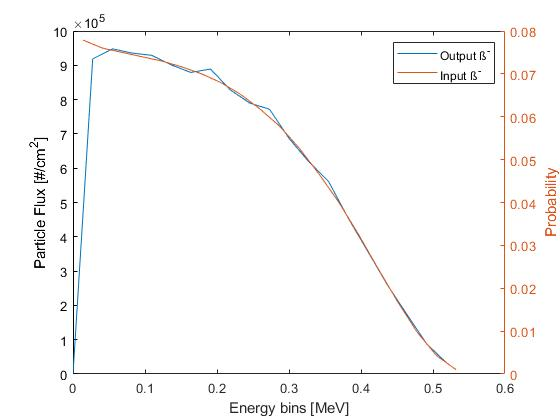
\includegraphics[scale=0.4]{Master Thesis Manuel Galdon/figures/Sr in VOID normalized to activity.jpg} 
        %\caption{Particle flux of \ce{^{90}Sr} in vacuum}
        \label{fig:Sr-90_VOID}
    \end{subfigure}
    \hspace{1cm}
    \begin{subfigure}{1 cm}
        \captionsetup{margin={0pt,-200pt}}
        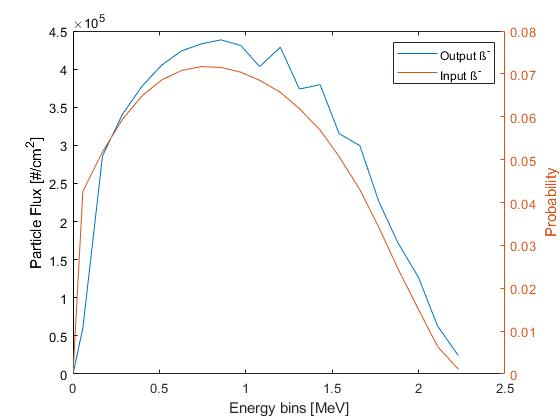
\includegraphics[scale=0.4]{Master Thesis Manuel Galdon/figures/Y in VOID normalized to activity.jpg}
        %\caption{Particle flux of \ce{^{90}Y} in vacuum}
        \label{fig:Y-90_VOID}
    \end{subfigure}
    \caption{Particle flux in vacuum of \ce{^{90}Sr} (left) and \ce{^{90}Y} (right).}
    \label{fig:particle_flux_VOID_Sr_and_Y}
\end{figure}

Theoretically, the output should be identical to the input spectrum. Even though there are no interactions to consider, the MCNP statistics might produce a small misalignment between the lines of both plots. It is important to mention that the simulated spectrum is obtained using histogram statistics in MCNP and it has required the data to be centered in the right energy bin. This correction is implemented beforehand by applying the relation $E_i = E_i + \frac{\Delta E}{2}$, where $E_i$ is each energy bin and $\Delta E$ is the difference between each bin and the up next. In the yttrium plot, a further correction is applied to improve the smoothness of the output. The result shows a fluctuation around 1 and 1.6 \unit{\mega\electronvolt} that comes from the statistics applied automatically by the simulation. This effect must be caused by the MCNP statistics and removing it by applying certain correction factors for visualisation purposes does not provide any further valuable insights into the understanding of the behaviour in vacuum.

In Figure \ref{fig:particle_flux_VOID_Sr_and_Y}, it is evident that the strontium spectrum lacks any photon emissions, which is expected since strontium decay does not produce photons. Due to the void geometry, there are no interactions between electrons and other particles, thereby ruling out the possibility of any secondary photon production under these conditions.

In contrast, the yttrium decay leads to a \textbf{single gamma} gamma photon emission at 1.76 \unit{\mega\electronvolt}, as specified in the source configuration. This photon is not shown on the graph because the probability is so low that the particle flux is barely noticeable when plotted along with the electron output.

A different behaviour becomes evident if all cells except those adjacent to the source are filled with air. In such case, there is production of secondary photons and, therefore, the electrons emitted by the source also decrease their intensity as many of them undergo the deflection that causes the \emph{bremsstrahlung}. 
\clearpage
The simulation result after running at $10^8$ particles is:

\begin{figure}[!h]
    \begin{subfigure}{7 cm}
        %\captionsetup{margin={20pt,0pt}}
        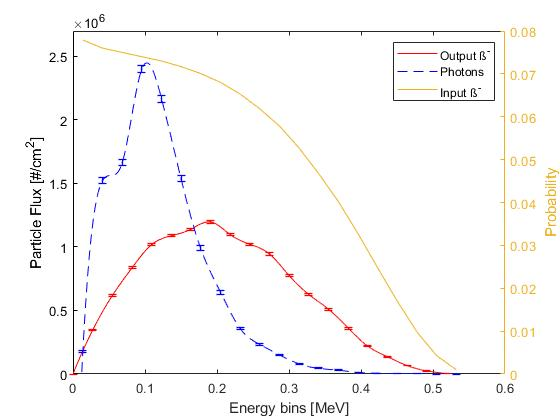
\includegraphics[scale=0.42]{Master Thesis Manuel Galdon/figures/Sr in air.jpg} 
        %\caption{Particle flux of \ce{^{90}Sr} in vacuum}
        \label{fig:Sr-90_air}
    \end{subfigure}
    \hspace{1cm}
    \begin{subfigure}{1 cm}
        \captionsetup{margin={0pt,-200pt}}
        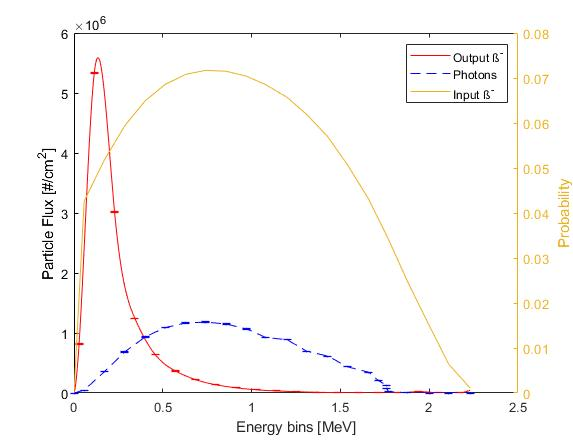
\includegraphics[scale=0.4]{Master Thesis Manuel Galdon/figures/Y in air.jpg}
        %\caption{Particle flux of \ce{^{90}Y} in vacuum}
        \label{fig:Y-90_air}
    \end{subfigure}
    \caption{Particle flux in air of \ce{^{90}Sr} (left plot) and \ce{^{90}Y} (right plot) against the energy bin. The right axis is the $\beta^-$ decay probability of strontium and yttrium in each energy bin, referred to as "Input $\beta^-$". These values serve as input for the \emph{SDEF} card of MCNP. The left axis is the particle flux i.e. intensity of the radiation measured in number of particles that move through each \unit{\square\centi\meter} of surface.}
    \label{fig:particle_flux_air_Sr_and_Y}
\end{figure}


In Figure \ref{fig:particle_flux_air_Sr_and_Y}, the particle flux has been normalized to the activity of the sample on the specified date, as mentioned after Equation \ref{eq:Activity of parent nucleus as a function of time}. To supplement representation of data, the electron output and photon flux have been interpolated using the \emph{spline} method. However, only the points that have an error bar are the actual data that the simulation returned. Here, the only data that has not been interpolated for practical reasons due to its values is the photon flux for yttrium, shown on the right graph.

Figure \ref{fig:particle_flux_air_Sr_and_Y} presents the photon outcomes for both samples. Unlike the vacuum scenario shown in Figure \ref{fig:particle_flux_VOID_Sr_and_Y}, it is observed that the flux is no longer negligible for the case of strontium. This change is attributed to the interaction of electrons with the dry air, as previously mentioned. Notably, the \emph{bremsstrahlung} production becomes more pronounced around 100 \unit{\kilo\electronvolt} and decreases rapidly after 150 \unit{\kilo\electronvolt}.

For yttrium, there is also \emph{bremsstrahlung} production in the low-energy region around 280 \unit{\kilo\electronvolt}. The energy that peaks above 0.35 particles per square centimeter corresponds to 1.76 \unit{\mega\electronvolt} and aligns with the discrete energy input bin specified in the input of MCNP.

In conclusion, the analysis of the \emph{bremsstrahlung} spectrum reveals the formation of secondary photons at various energy levels. The spectrum of the incident electron with energies of 100 \unit{\kilo\electronvolt}, 150 \unit{\kilo\electronvolt}, and 280 \unit{\kilo\electronvolt} exhibit distinctive secondary photon peaks, each reflecting specific energy interactions between the incident electrons and the surrounding air. The secondary photons formed are predominantly X-rays with the exception of the \emph{gamma} photons of the order of \unit{\mega\electronvolt} that is produced directly in the yttrium sample and is, therefore, not part of the \emph{bremsstrahlung} spectrum.

Lastly, for comparison purposes, the spectrum of both samples according to the live chart of Nuclides from the \emph{International Atomic Energy Agency} is presented in the next figure. According to \textit{Laboratory, L.A.N.: International Atomic Energy Agency} \cite{intlAtomicEnergy}, the spectrum is:

\begin{figure}[!h]
    \begin{subfigure}{6 cm}
        %\captionsetup{margin={20pt,0pt}}
        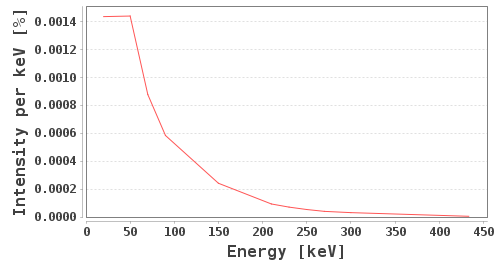
\includegraphics[scale=0.6]{Master Thesis Manuel Galdon/figures/Sr BS spectrum.png} 
        %\caption{Particle flux of \ce{^{90}Sr} in vacuum}
        \label{fig:Sr BS spectrum}
    \end{subfigure}
    \hspace{1cm}
    \begin{subfigure}{1 cm}
        \captionsetup{margin={0pt,-200pt}}
        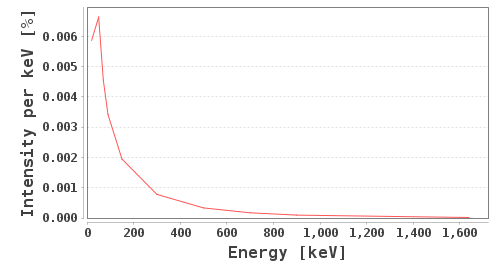
\includegraphics[scale=0.605]{Master Thesis Manuel Galdon/figures/Y BS spectrum.png}
        %\caption{Particle flux of \ce{^{90}Y} in vacuum}
        \label{fig:Y BS spectrum}
    \end{subfigure}
    \caption{Bremsstrahlung spectrum of \ce{^{90}Sr} (left) and \ce{^{90}Y} (right)}
    \label{fig:spectrum of Sr and Y}
\end{figure}

In the right plot, the spectrum is divided into energy bins ranging from 0 to 2.3 \unit{\mega\electronvolt}, with corresponding intensities. Notably, the breaking radiation of yttrium has a higher intensity in the lower energy ranges (40-100 \unit{\kilo\electronvolt}), demonstrating a decreasing trend as energy increases. This matches the expected behavior of \emph{bremsstrahlung} radiation and the result presented in this subsection. The photon particle flux is higher in the lower energy region and almost negligible for the higher energies. The same conclusion is reached for the strontium. In this case, the maximum intensity agrees with the simulated spectrum shown in Figure \ref{fig:particle_flux_air_Sr_and_Y}.% as the line for the photon radiation peaks in the same energy ranges where in Figure \ref{fig:spectrum of Sr and Y} the highest values are located.

%The reason why the elements show the highest emission of radiation at certain energies is because the cross section of the electrons is higher for those E values.

Finally, the check source is configured in MCNP according the probabilities calculated earlier in this chapter, the geometry and relative positions of the source and the chamber, and the breaking radiation spectrum discussed in this last section. 